\documentclass{beamer}
\usepackage{appendixnumberbeamer}

\mode<presentation>{\usetheme[subsectionpage=progressbar,block=fill,numbering=none]{metropolis}}

\usepackage[sfdefault]{FiraSans} %% option 'sfdefault' activates Fira Sans as the default text font
\usepackage[english]{babel}
\usepackage[utf8]{inputenc}

\usepackage{graphicx} % Allows including images
\usepackage{pgfplots}
\usepackage{caption}
\usepackage{booktabs} % Allows the use of \toprule, \midrule and \bottomrule in tables
\usepackage{multicol}

% Math packages
\usepackage{amsmath}
\usepackage{mathtools}
\usepackage{amssymb}
\usepackage{mathpartir}
\usepackage{stmaryrd}
\usepackage{centernot}
\usepackage[normalem]{ulem}
\usepackage[absolute,overlay]{textpos}

%% Coding
%\usepackage[outputdir=build]{minted}
\usepackage{listings}
\lstdefinelanguage{cyp}{
  keywords={Lemma,goal,Proof,QED,To,show,Case},
  keywordstyle=\color{blue}\bfseries,
  keywords=[2]{data},
  keywordstyle=[2]{\color{purple}\bfseries},
  keywords=[3]{.=.},
  keywordstyle=[3]{\color{red}\bfseries},
  comment=[l]{--},
  commentstyle=\color{purple}\ttfamily,
}

\lstset{
  language=cyp,
  extendedchars=true,
  basicstyle=\ttfamily,
  showstringspaces=false,
  showspaces=false,
  tabsize=2,
  breaklines=true,
  showtabs=false
}

% Coloured boxes
\usepackage{tcolorbox}
\colorlet{alert}{mLightBrown}
\colorlet{mLightBrownTransparent}{white!70!mLightBrown}
\newtcolorbox{alertbox}
{standard jigsaw, opacityback=0,colframe=alert}
\newtcolorbox{tbox}
{standard jigsaw, opacityback=0,opacityframe=0}

% \newcommand{\haskell}[1]{\mintinline{haskell}{#1}}

\title{Engaging, Large-Scale Functional Programming Education in Physical and Virtual Space} % the title on the title page

\author{\underline{Kevin Kappelmann}, \underline{Jonas Rädle}, Lukas Stevens} % Your name
\institute[TU Munich]{Technical University of Munich}
\date{March 16, 2022} % Date, can be changed to a custom date

\begin{document}

\maketitle

\begin{frame}
Supported by
\begin{itemize}
  \item Lecturer: Tobias Nipkow
  \item Manuel Eberl
  \item 2019: 13 student assistants
  \item 2020: 22 student assistants
\end{itemize}
\end{frame}

%------------------------------------------------
\section{Challenges}
% Soaring Enrolments
\begin{frame}{Soaring Enrolments}
\only<1>{\centerline{\Large{\alert{1. Number of Computer Science students exploded}}}}
\only<2->{\centerline{Example: Computer Science at TU Munich}

\pause
\begin{multicols}{2}
\begin{figure}
\centering
\captionsetup{justification=centering}
% somehow this needs to be 1.02 when it is 1 below
\resizebox{1.03\linewidth}{!}{
\begin{tikzpicture}
\begin{axis}[
    ymin=0,
    x tick label style={/pgf/number format/.cd,%
      set thousands separator={}}
  ]
  \addplot +[color=red, mark options={fill=red}] coordinates {
    (2013, 3555)
    (2014, 3815)
    (2015, 4240)
    (2016, 4744)
    (2017, 5399)
    (2018, 5986)
    (2019, 6458)
    (2020, 7444)
    (2021, 8253)
  };
\end{axis}
\end{tikzpicture}
}
\caption*{Number of CS students\\(132\% increase)}
\end{figure}

\columnbreak

\begin{figure}
\centering
\captionsetup{justification=centering}
\resizebox{\linewidth}{!}{
\begin{tikzpicture}
\begin{axis}[
    ymin=0,
    x tick label style={/pgf/number format/.cd,%
      set thousands separator={}}
  ]
  \addplot coordinates {
    (2013, 439)
    (2014, 449)
    (2015, 432)
    (2016, 436)
    (2017, 438)
    (2018, 450)
    (2019, 500)
    (2020, 529)
    (2021, 573)
  };
\end{axis}
\end{tikzpicture}
}
\caption*{Number of CS academic staff (31\% increase)}
\end{figure}
\end{multicols}
}
\visible<3>{\centerline{\Large{\alert{1000+ students per course are the new normal}}}}
\end{frame}

\begin{frame}{The Pandemic}
\only<1>{\centerline{\Large{\alert{2. Radical transition to online classes}}}}
\only<2>{\centerline{How can we go from here\dots}
\begin{figure}
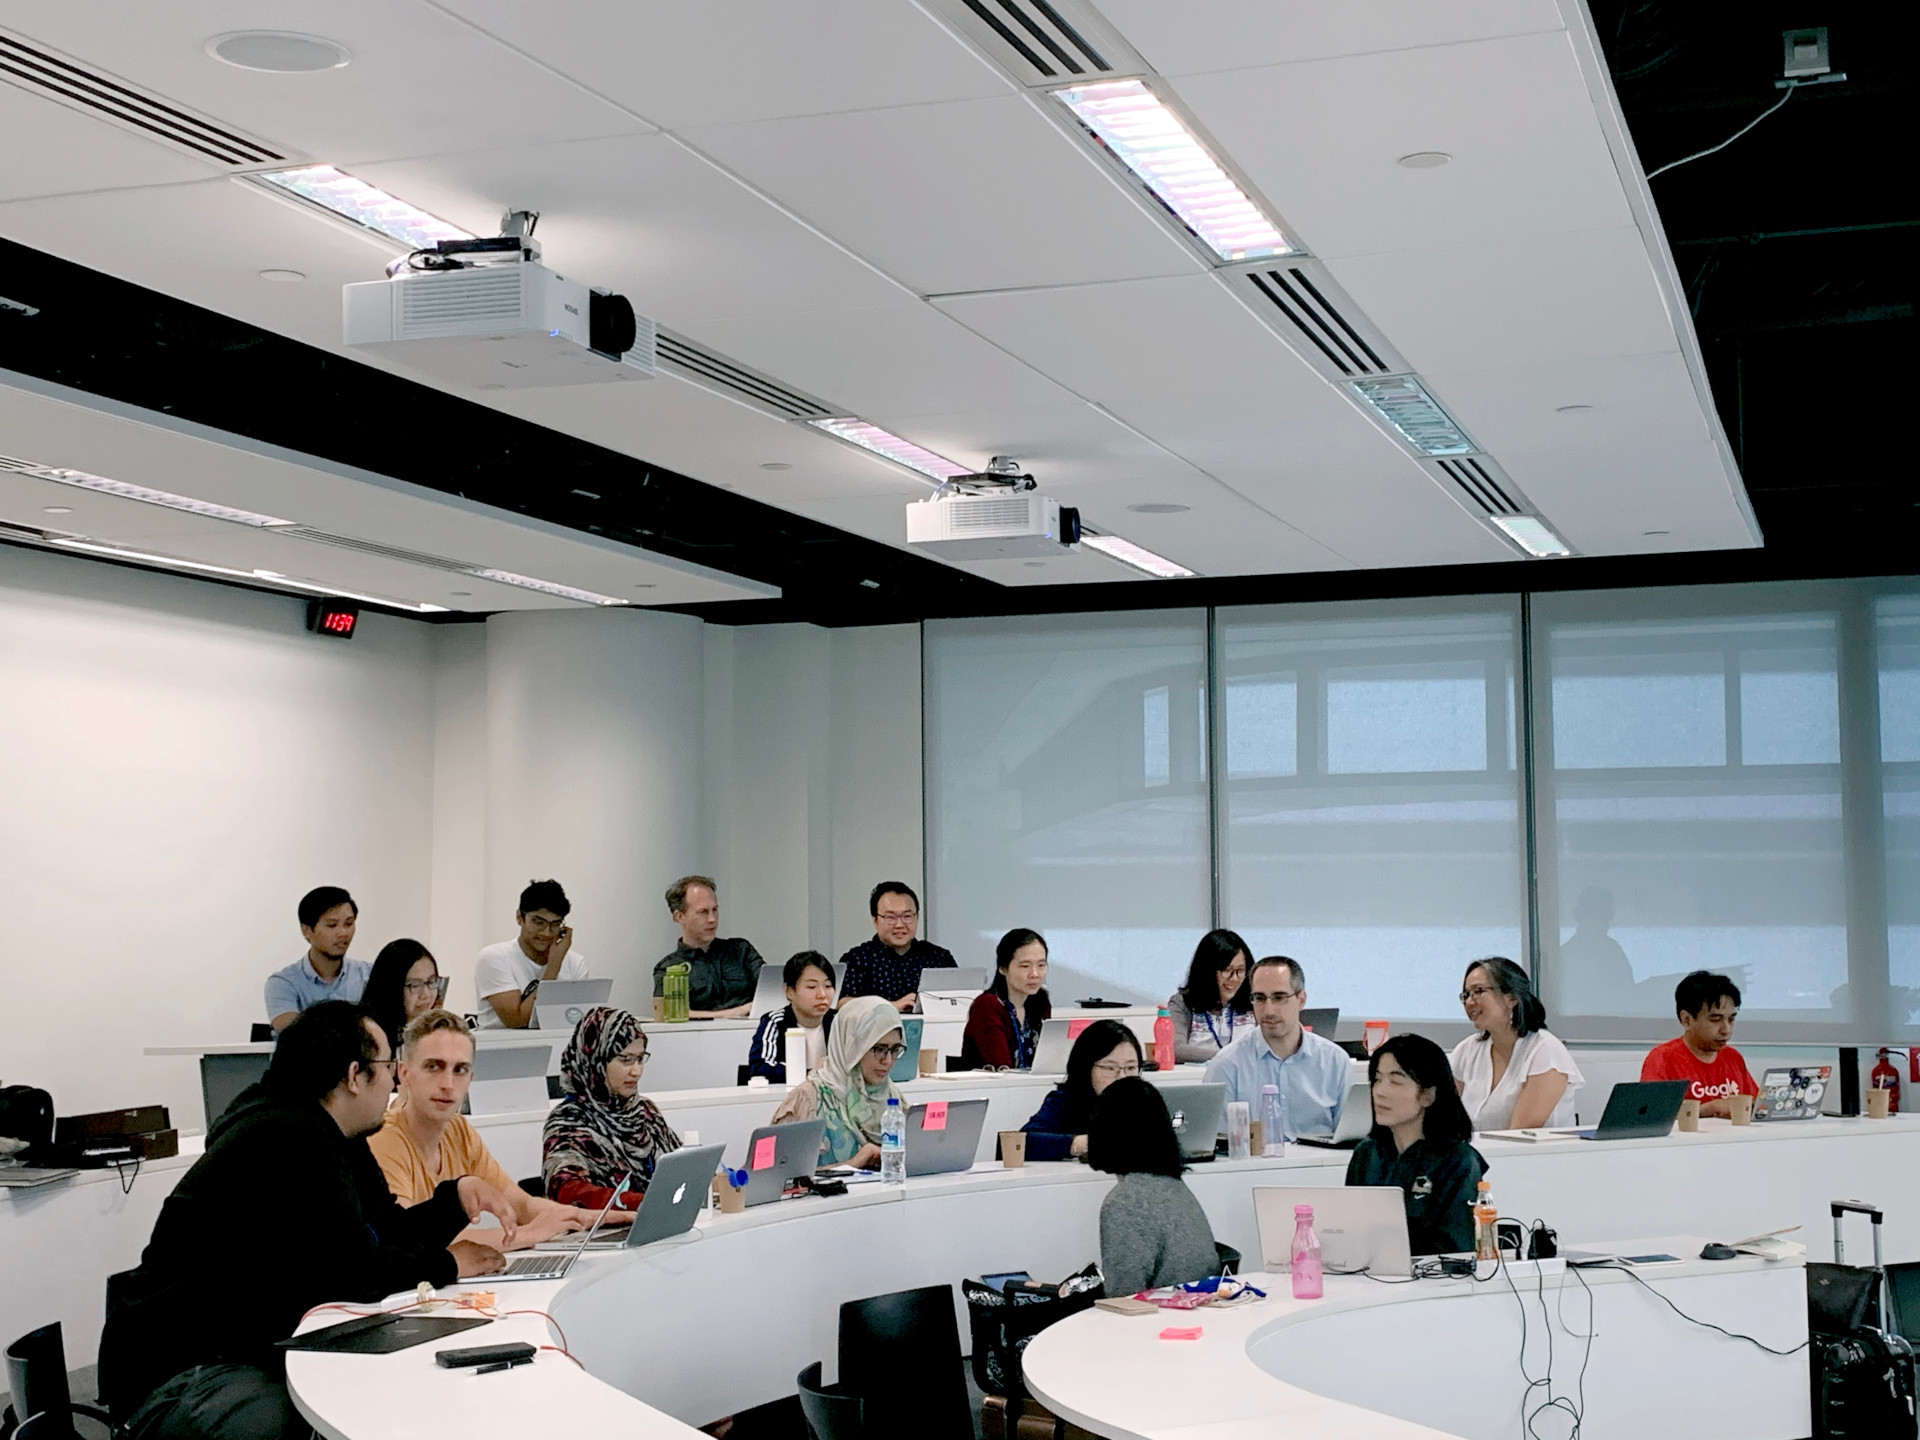
\includegraphics[width=0.75\linewidth]{assets/class}
\end{figure}
}
\only<3>{\centerline{to here\dots}
\begin{figure}
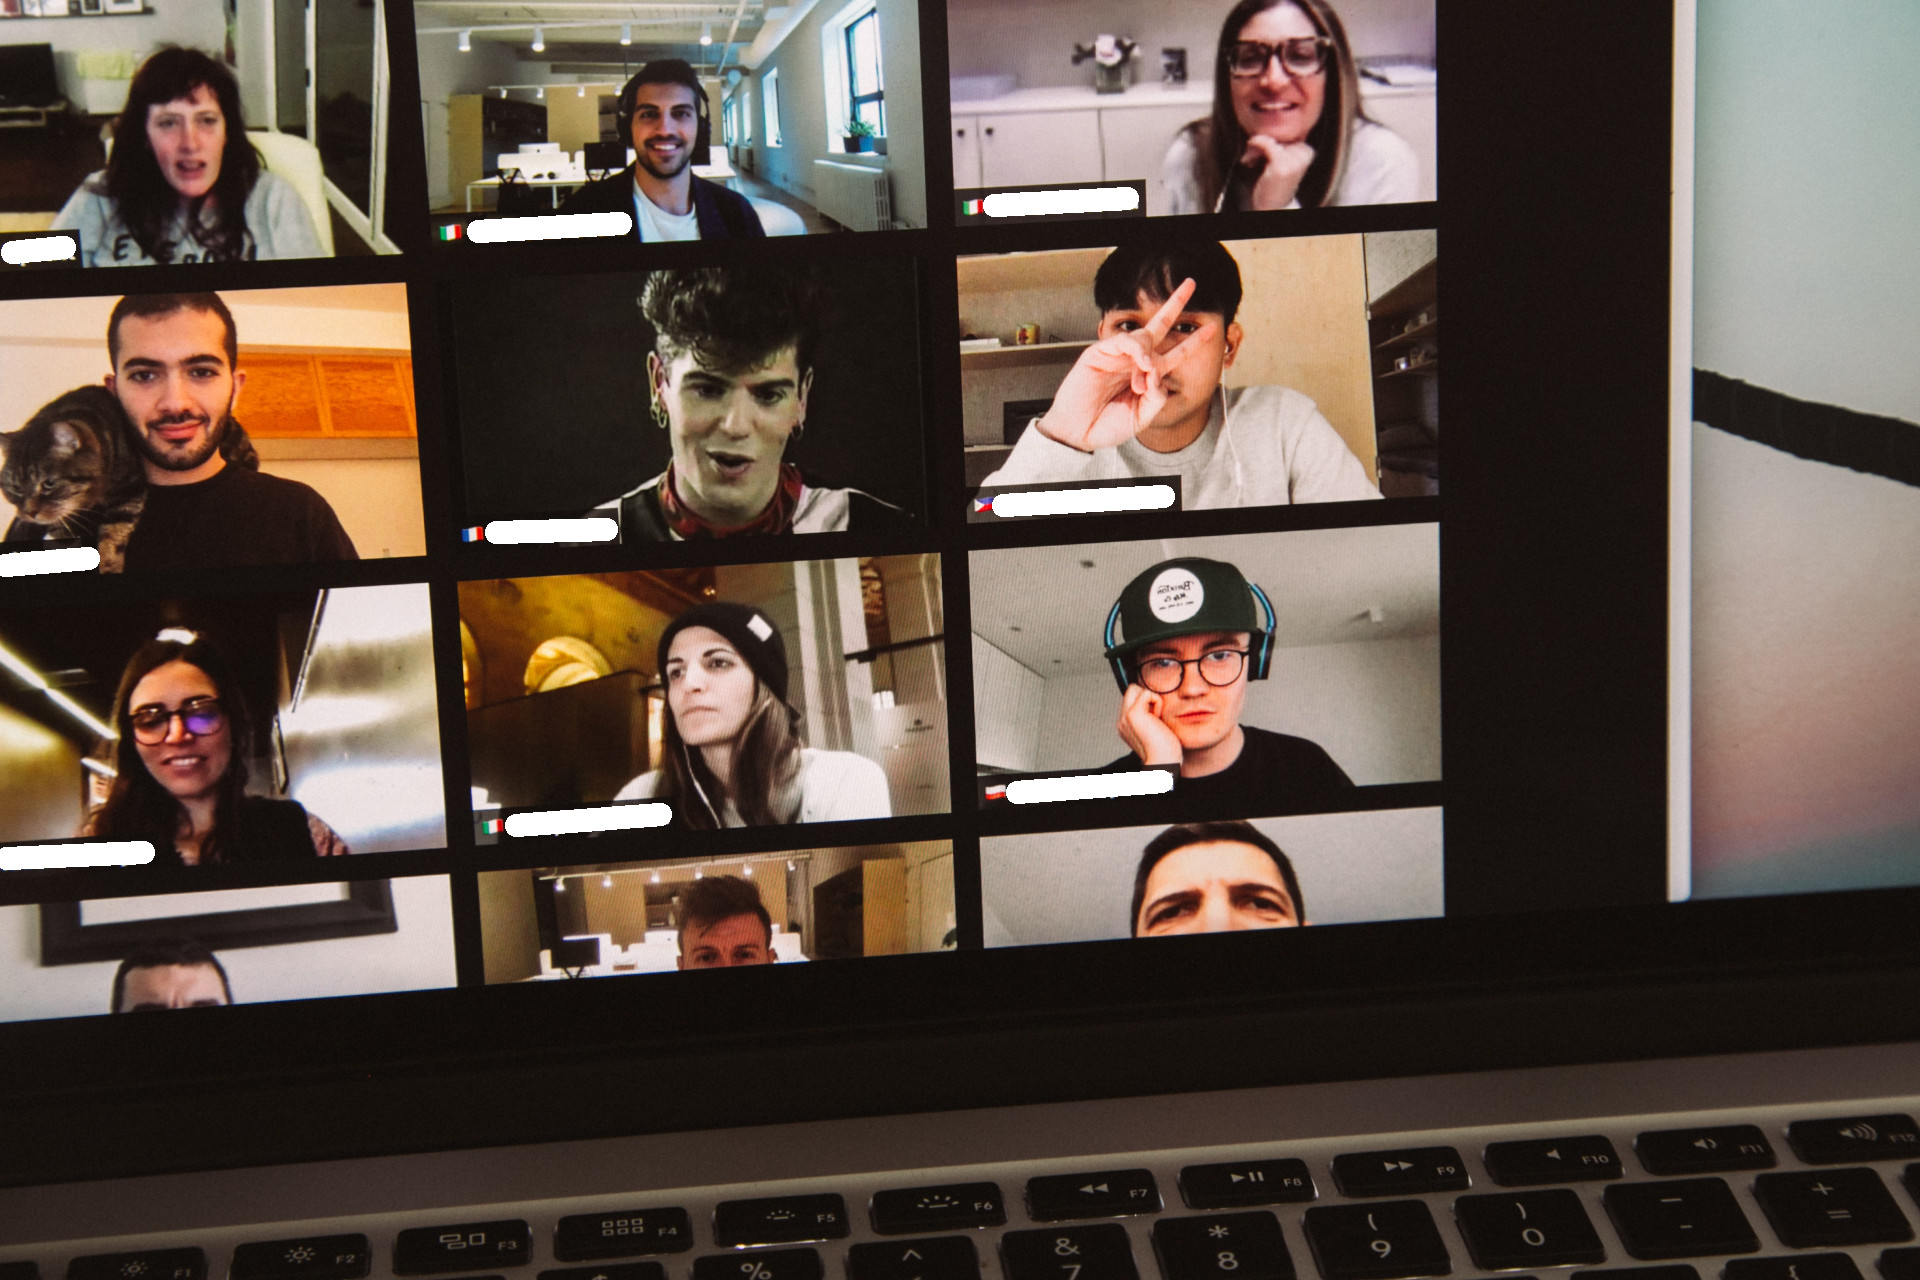
\includegraphics[width=0.85\linewidth]{assets/zoom}
\end{figure}
}
\only<4>{\centerline{without ending up here?}
\begin{figure}

\includegraphics[width=0.85\linewidth]{assets/zoom_fatigue}
\end{figure}
}
\end{frame}

\begin{frame}{Usefulness of Functional Programming}
\only<1>{
\centering\Large{\alert{3. Students question the usefulness of functional languages beyond academia}}}
\only<2>{
\begin{multicols}{2}

\begin{figure}

\includegraphics[width=0.8\linewidth]{assets/xkcd_haskell}
\caption*{\url{xkcd.com/1312}}
\end{figure}

\columnbreak

\begin{figure}

\includegraphics[width=0.8\linewidth]{assets/xkcd_tailrec}
\caption*{\url{xkcd.com/1270}}
\end{figure}
\end{multicols}
}
\end{frame}

\begin{frame}
\centerline{\alert{\huge{There is hope!}}}
\begin{itemize}[<+->]
\item We managed to cope with all these challenges
\item We share our insights, tools, and exercises for other educators
\end{itemize}

\visible<2->{
  You can find our resources on:\\
  \centerline{\small\url{github.com/kappelmann/engaging-large-scale-functional-programming}}
}

\vspace{\baselineskip}
\visible<3->{
Note: We used Haskell, but most ideas apply to any functional programming course
}
\end{frame}

%------------------------------------------------
% \section{Course Structure and Conditions}
% \begin{frame}{Hard Facts}
% \begin{itemize}[<+->]
  % \item Typical functional programming introductory course\\
    % Special: Formal proofs and proof checker
  % % \item 5 ECTS course (${\sim}150$ hours of work)
  % \item 14 weeks; each week: one 90-minute lecture, one 90-minute tutorial, and one homework sheet
  % % \item Students took courses on Java, algorithms and data structures, discrete mathematics, and linear algebra.
   % \item Winter semester 2019: 1057 students and 13 student assistants\\
     % Winter semester 2020 (online): 1031 students and 22 student assistants
% \end{itemize}
% \end{frame}

% \begin{frame}{Syllabus Excerpt}
% We used Haskell, but most ideas apply to other functional languages.
% \pause
% \begin{itemize}[<+->]
  % \item Basic FP concepts: recursion and pattern matching (numbers and lists), polymorphism
  % \item Formal proofs by structural and computation induction
  % \item More FP concepts: higher-order functions, type classes, algebraic datatypes
  % \item Specifics: modules, IO, lazy evaluation, tail recursion
% \end{itemize}
% \end{frame}

%------------------------------------------------
% \section{Lectures}
% \begin{frame}{Time Is Short}
  % \centerline{\alert{\Large{See our paper ;)}}}
% \end{frame}


%------------------------------------------------
\section{Practical Part}
\subsection{Engagement Mechanisms}
\begin{frame}{Grade Bonus}
\centerline{\Large{\alert{Incentives do work!}}}
\pause
\begin{itemize}[<+->]
\item Bonus of one grade step on final exam if certain goals are achieved
\item Offer multiple ways to obtain points: homework exercises, participation in workshops, programming contests,\dots
\item Was once abolished\dots\\
\item[] Result: number of homework submissions severely decreased
\end{itemize}
\end{frame}

\begin{frame}{Instant Feedback}
\centerline{\Large{\alert{Feedback must come fast!}}}
\pause
\begin{itemize}[<+->]
\item Asynchronous Q\&A forum
\item Automated testing and feedback
\begin{itemize}
  \item \emph{ArTEMiS} runs tests, balances loads, offers exam mode,\dots
  \item \emph{Tasty} combines QuickCheck, SmallCheck, and HUnit tests
  \item \emph{Check Your Proof} for automated proof checking
\end{itemize}
\item Manual reviews turned out to be inefficient\dots
\begin{itemize}
  \item \emph{HLint} offers feedback more directly
  \item Student assistants create engaging exercises instead
\end{itemize}
\end{itemize}
\end{frame}

\begin{frame}{Workshops With Industry Partners}
\vspace{\baselineskip}

\centerline{\Large{\alert{Functional programming is practical!}}}
\pause
\begin{itemize}
\item In 2020, we hosted 3 workshops with industry partners
\begin{enumerate}[<3->]
  \item Design patterns for functional programs
  \item Networking and advanced IO
  \item User interfaces and functional reactive programming
\end{enumerate}
\item<4-> Great success: 120 registrations for 105 spots
\item<5-> In some cases, workshop extended for multiple hours
\item<6-> Little organisational work
\end{itemize}
\end{frame}
% \begin{frame}{Workshops With Industry Partners}
% \vspace{\baselineskip}

% \centerline{\Large{\alert{Functional programming is practical!}}}
% \pause
% \begin{itemize}
% \visible<2->{
% \item In 2020, we hosted three workshops}
% % \begin{enumerate}
  % % \item Design patterns for functional programs
  % % \item Networking and advanced IO
  % % \item User interfaces and functional reactive programming
% % \end{enumerate}
% \only<6->{
% \visible<6->{
% \item Great success: 120 registrations for 105 spots}
% \visible<7->{
% \item In some cases, workshop extended for multiple hours}
% \visible<8->{
% \item Little organisational work}}
% \end{itemize}
% \only<1-5>{\vspace{-\baselineskip}}
% \only<1-3>{
% \visible<3>{
% \centering
% 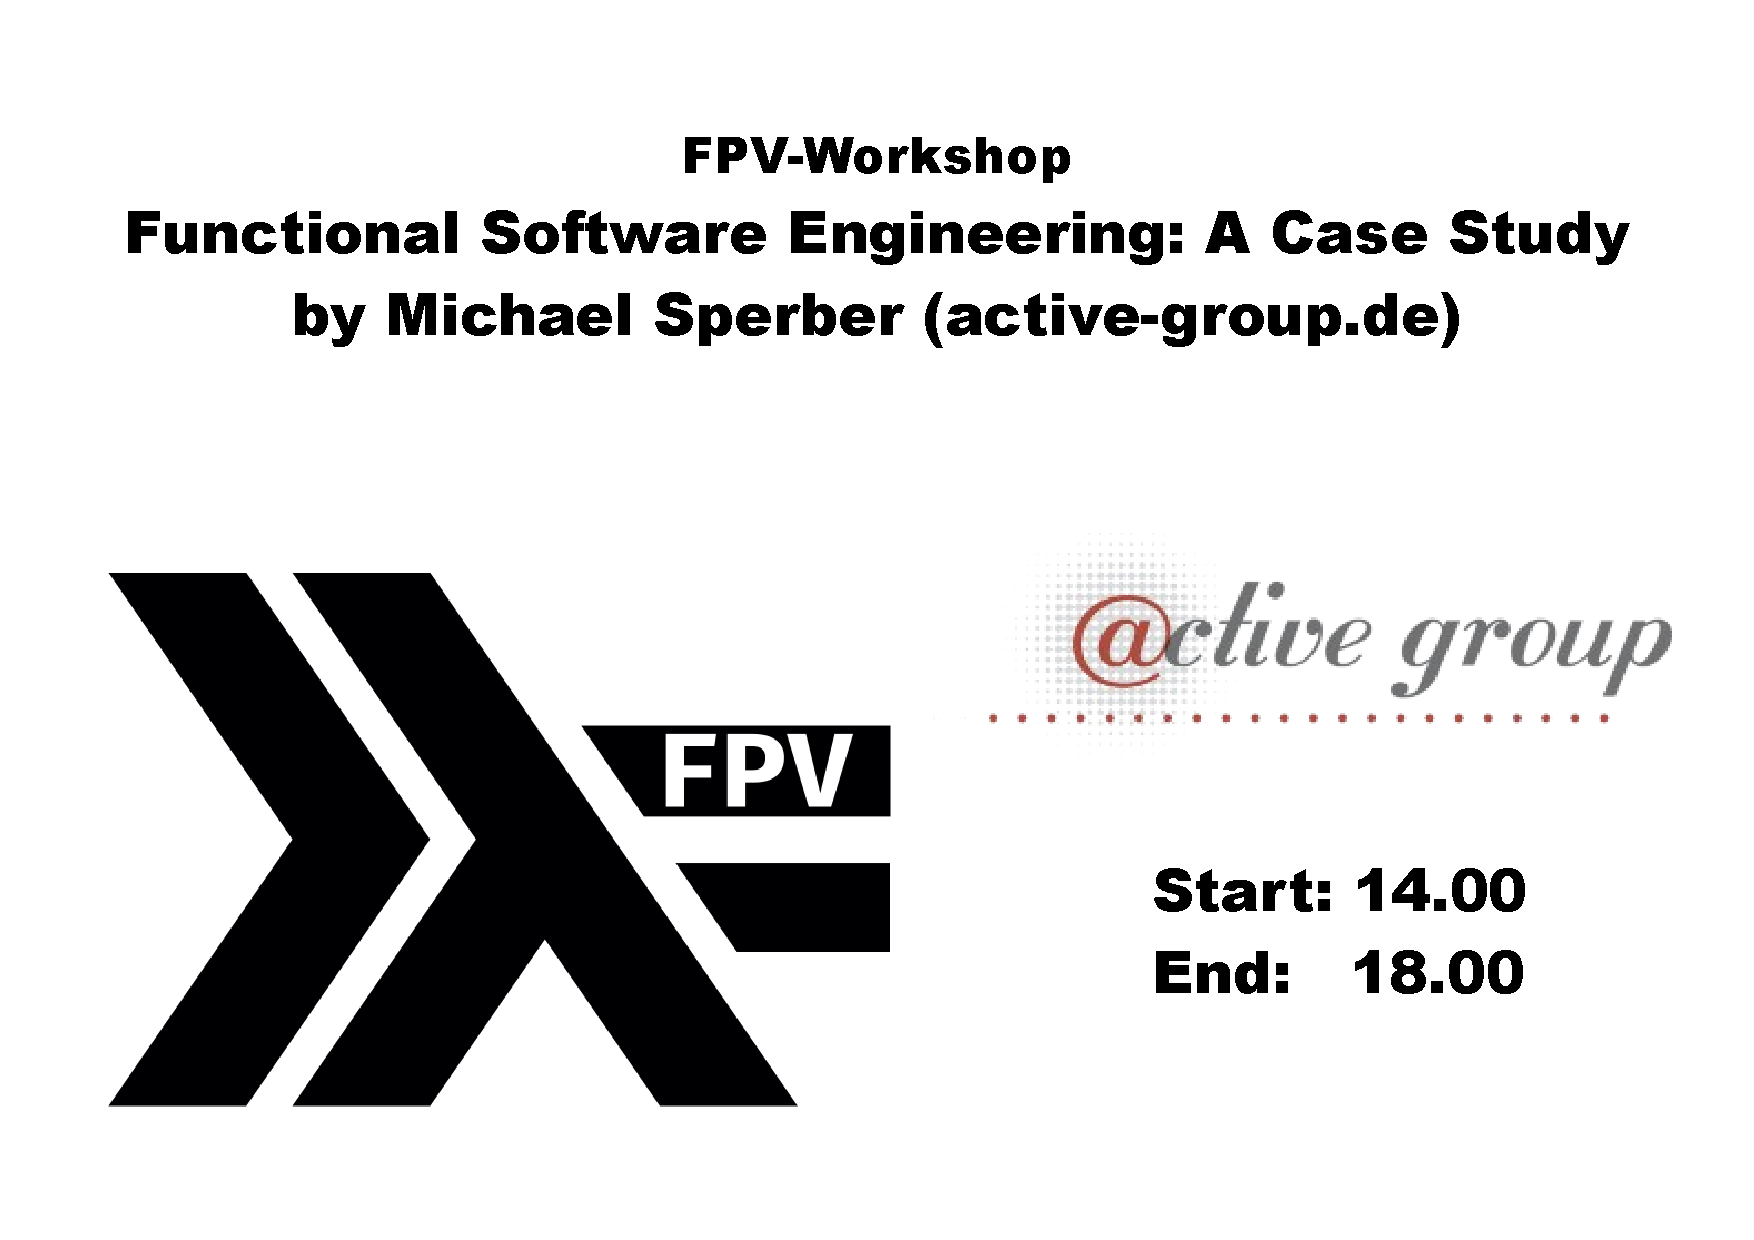
\includegraphics[width=0.9\linewidth]{assets/workshop_slide_active_group.pdf}}}
% \only<4>{
% \centering
% 
\includegraphics[width=0.9\linewidth]{assets/workshop_slide_networking.pdf}}
% \only<5>{
% \centering
% 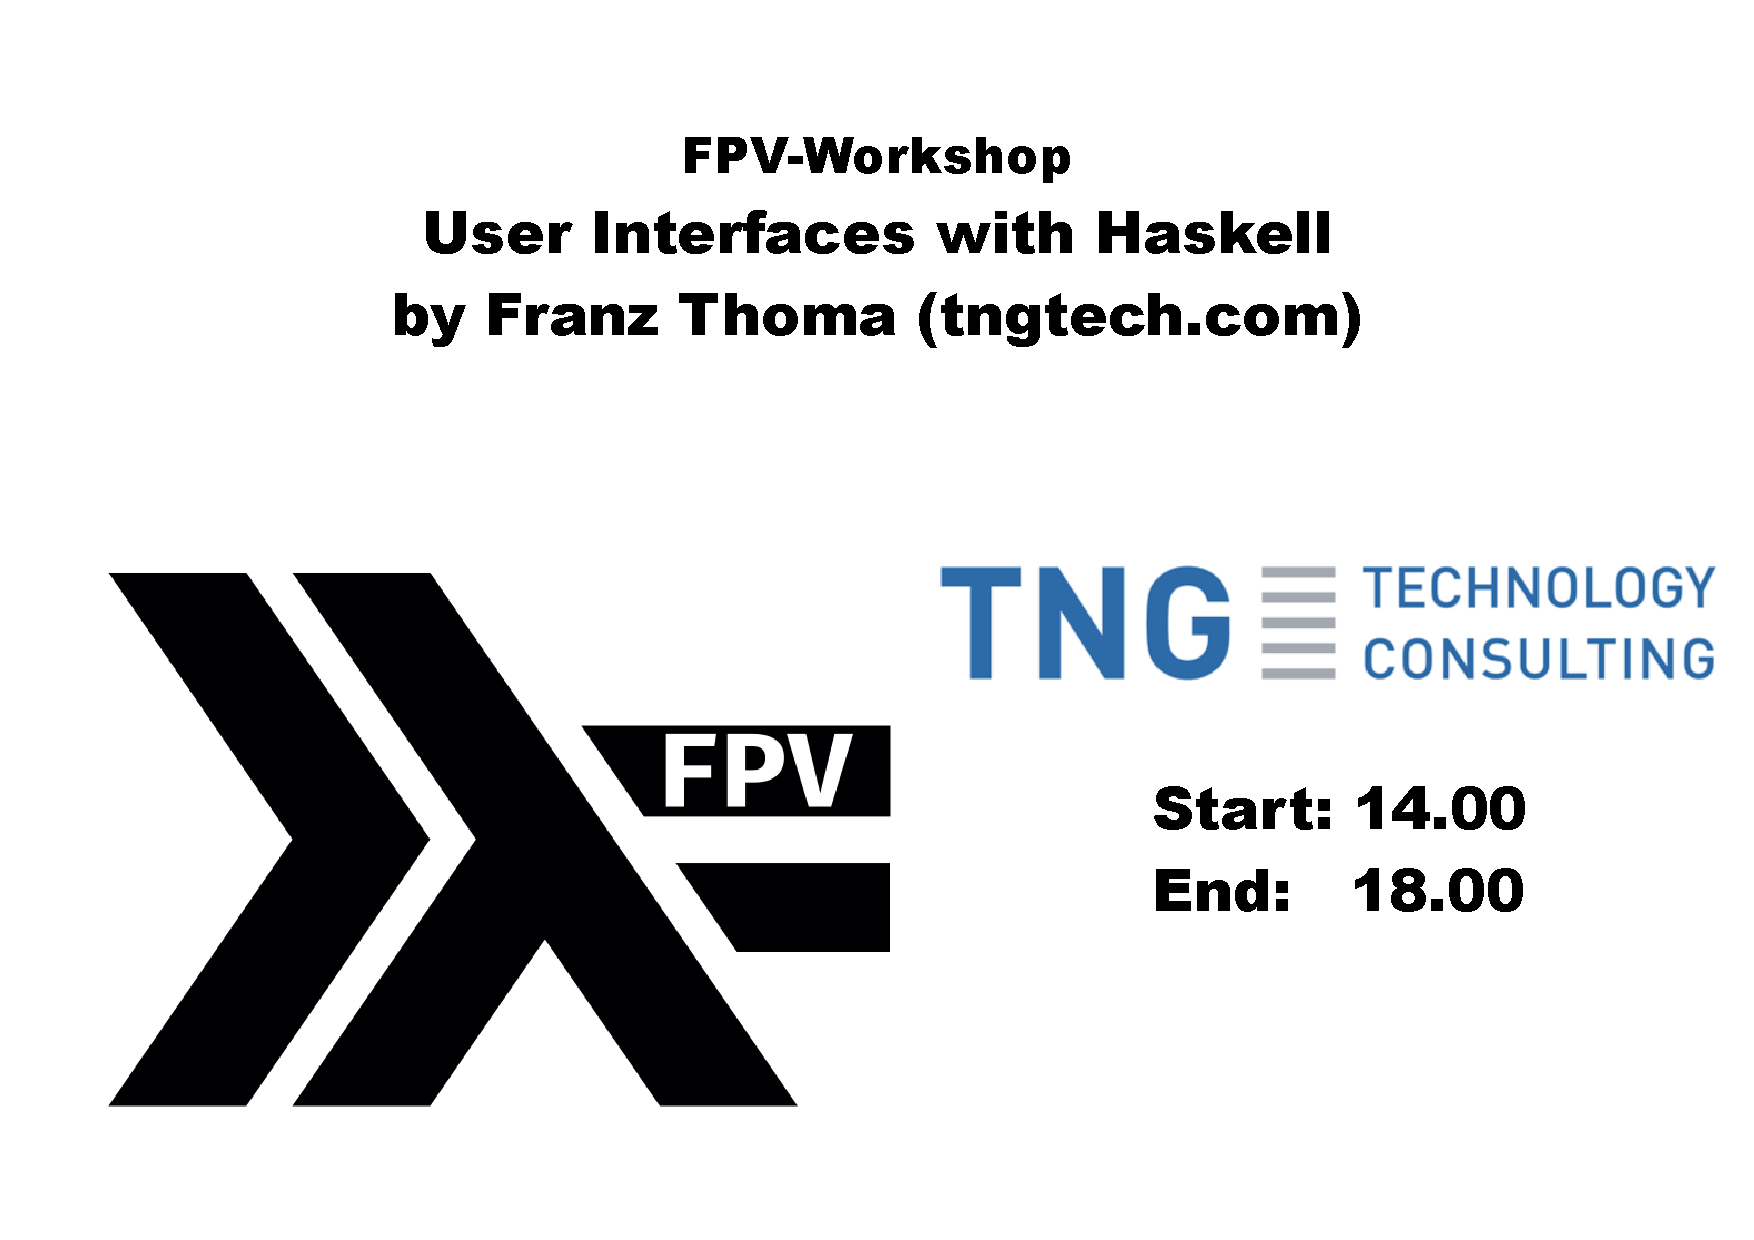
\includegraphics[width=0.9\linewidth]{assets/workshop_slide_ui.pdf}}
% \end{frame}

\begin{frame}{Social Interactions}
\centerline{\Large{\alert{The social environment matters!}}}
\pause
\begin{itemize}[<+->]
% \item Truism: students spend more time on courses they like
\item Online courses are isolating\dots
\item[] so let us foster social interaction:
\begin{itemize}[<4->]
  \item Pair-programming in tutorials
  \item ACM-ICPC-like programming contest
  \item Get-together hangout sessions
  \item Award ceremonies
\end{itemize}
\end{itemize}
\end{frame}

\begin{frame}[fragile]{Competitions}
\centerline{\Large{\alert{Offer challenges to go beyond the syllabus!}}}
\pause
\begin{itemize}[<+->]
\item Diverse, weekly competition exercises
\end{itemize}
\end{frame}

%------------------------------------------------
\begin{frame}[fragile]{Competitions}
\begin{onlyenv}<1>

\centerline{Code Golf}
\vspace{15pt}
\tiny
\begin{lstlisting}
numberToEo = unwords <<< catMaybes <<< reverse <<< flip lookup `zipWith` table <<< chunksOf 3 <<< pack <<< reverse
\end{lstlisting}
\begin{lstlisting}
topCycle = concatMap snd . ap zip (iterate . fmap nub . concatMap . dominators <*> copeland)
\end{lstlisting}
\begin{lstlisting}
traceFractran rs n = n : fromMaybe [] (traceFractran rs <$> numerator <$> (liftM2 eqInteger truncate numerator) `find` map (fromIntegral n *) rs)
\end{lstlisting}
\begin{lstlisting}
bernoulli = genericIndex $ map head $ iterate ((*) `zipWith` enumFrom 1 <<< zipWith subtract `ap` tail) $ recip `map` enumFrom 1
\end{lstlisting}




\end{onlyenv}
\only<2>{\centerline{Optimization}
\begin{figure}
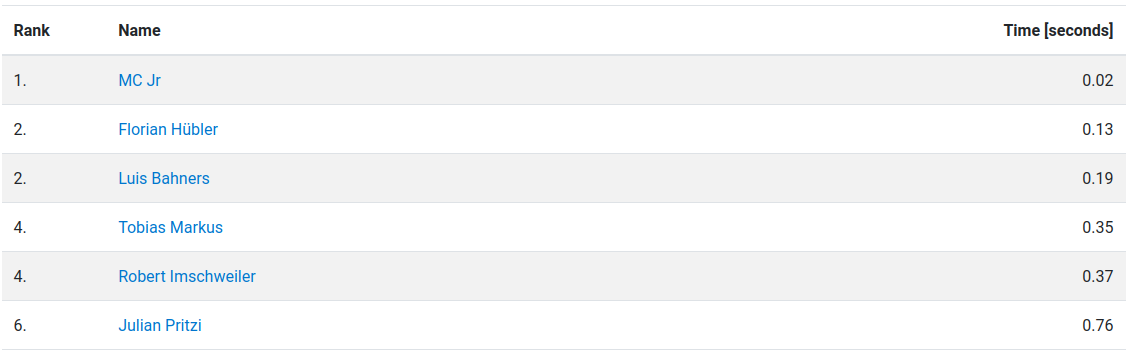
\includegraphics[width=0.85\linewidth]{assets/optimization}
\end{figure}
}
\only<3>{\centerline{Strategy}
\begin{figure}
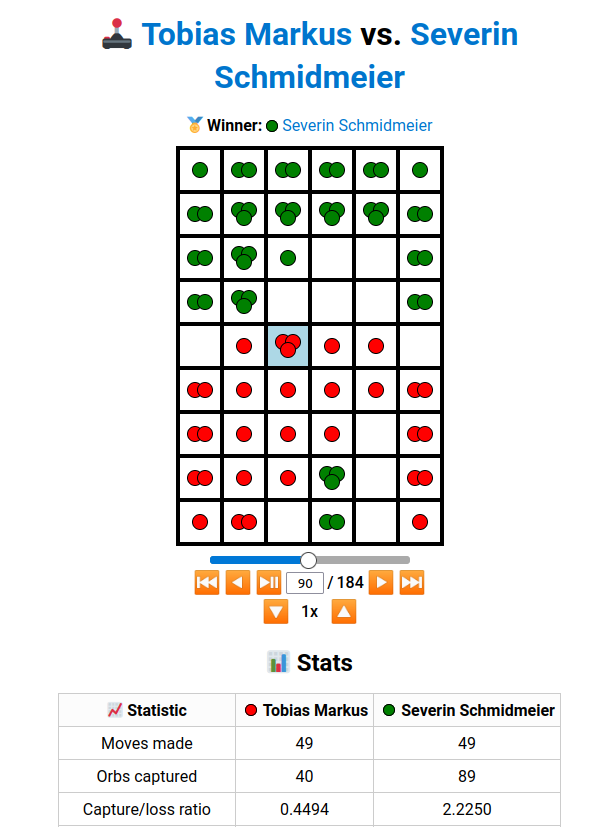
\includegraphics[height=0.85\textheight]{assets/strategy}
\end{figure}
}
\only<4>{\centerline{Creativity}
\begin{figure}

\includegraphics[height=0.85\textheight]{assets/creativity}
\end{figure}
}
\only<5>{\centerline{Creativity}
\begin{figure}
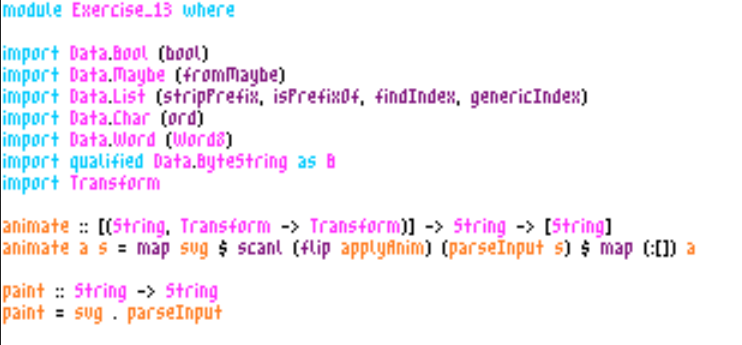
\includegraphics[width=0.85\linewidth]{assets/creativity2}
\end{figure}
}
\end{frame}

\begin{frame}[fragile]{Competitions}
\centerline{\Large{\alert{Offer challenges to go beyond the syllabus!}}}
\begin{itemize}
\item Diverse, weekly competition exercises
% \begin{itemize}[<3->]
  % \item Code-golfing
  % \item Optimisations (SAT and resolution provers, mathematical computations,\dots)
  % \item Games strategies and tournaments
  % \item Creative tasks: art and music generation
% \end{itemize}
% \item Accompanied by humorously written blog posts
\item Awards for top 30 students
\item<2-> Works extremely well to motivate talented students\dots
\item[]<3-> \emph{but it is very time-consuming}.
\end{itemize}
% \begin{onlyenv}<2>
% \begin{minted}[fontsize=\small]{haskell}
% bernoulli = genericIndex $ map head $ iterate
  % ((*) `zipWith` enumFrom 1 <<< zipWith subtract =<< tail)
  % recip `map` enumFrom 1
% \end{minted}
% \end{onlyenv}
\end{frame}



%------------------------------------------------
\section{Check Your Proof}

\begin{frame}{CYP In A Nutshell}

\begin{itemize}[<+->]
  \item Operates on a strict, untyped subset of Haskell
  \item Automatically checks simple inductive proofs
  \item Provides instant feedback
  \item Integrates with Tasty
\end{itemize}
\end{frame}

\begin{frame}[fragile]{Background Theory}
\lstset{language=CYP}
  \begin{lstlisting}
data List a = [] | a : List a

[] ++ ys = ys
(x : xs) ++ ys = x : (xs ++ ys)

goal xs ++ (ys ++ zs) .=. (xs ++ ys) ++ zs
  \end{lstlisting}
\end{frame}

\begin{frame}[fragile]{The \texttt{[]} Case}
  \begin{lstlisting}
Lemma: xs ++ (ys ++ zs) .=. (xs ++ ys) ++ zs
Proof by induction on List xs
  Case []
    To show: [] ++ (ys ++ zs) .=. ([] ++ ys) ++ zs
    Proof
                      [] ++ (ys ++ zs)
      (by def ++) .=. ys ++ zs
      (by def ++) .=. ([] ++ ys) ++ zs
    QED
  \end{lstlisting}
\end{frame}

\begin{frame}[fragile]{The \texttt{Cons} Case}
  \begin{lstlisting}
  Case x : xs
    To show: (x : xs) ++ (ys ++ zs)
         .=. ((x : xs) ++ ys) ++ zs
    IH: xs ++ (ys ++ zs) .=. (xs ++ ys) ++ zs
    Proof
                        (x : xs) ++ (ys ++ zs)
      (by def ++)   .=. x : (xs ++ (ys ++ zs))
      (by IH)       .=. x : ((xs ++ ys) ++ zs)

                        ((x : xs) ++ ys) ++ zs
      (by def ++)   .=. (x : (xs ++ ys)) ++ zs
      (by def ++)   .=. x : ((xs ++ ys) ++ zs)
    QED
QED
  \end{lstlisting}
\end{frame}

\begin{frame}{Our Experience With CYP}
\begin{itemize}[<+->]
  \item Student feedback 18 positive, 3 negative
  \item Main criticism: lack of documentation
  \item Mostly well-structured inductive proofs in the exam
\end{itemize}
\end{frame}


\begin{frame}
\centerline{\alert{\huge{Find more in our repository!}}}
\begin{itemize}
\item IO mocking framework
\item ACM-ICPC-like programming contest framework
\item A music synthesiser
\item More engagement mechanisms and insights, our technical setup,\dots
\end{itemize}

\vspace{\baselineskip}
\centerline{\small\url{github.com/kappelmann/engaging-large-scale-functional-programming}}
\end{frame}



%------------------------------------------------
\section{Future Work}

\begin{frame}{Future Work}
\centerline{Preventing collaboration/cheating}
\begin{figure}
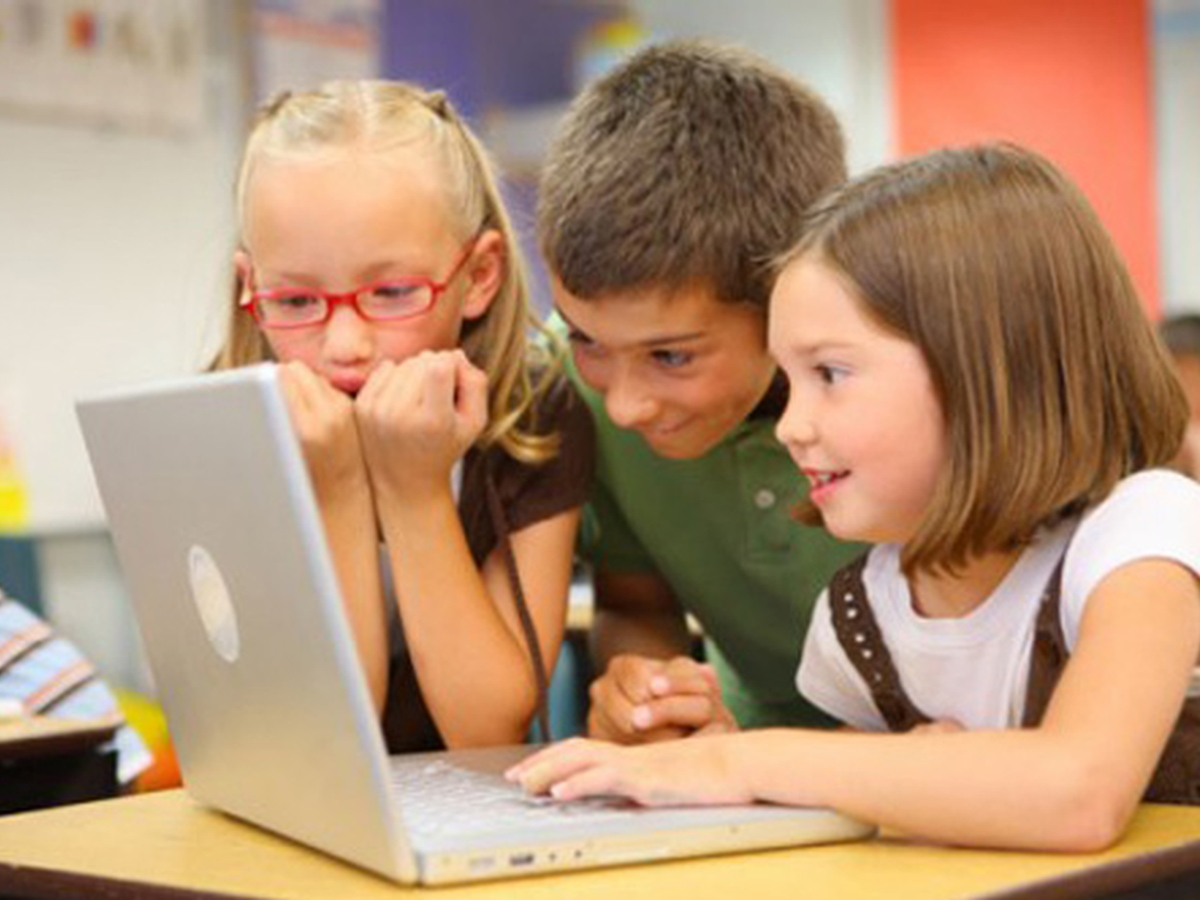
\includegraphics[width=0.85\linewidth]{assets/group}
\end{figure}
\end{frame}

%------------------------------------------------
\begin{frame}[standout]
\Large{\alert{Any questions?}}

\end{frame}
%----------------------------------------------------------------------------------------
%\begin{frame}[allowframebreaks]{References}
  %\bibliography{../paper/sources.bib}
  %\bibliographystyle{abbrv}
%\end{frame}

% \begin{frame}[allowframebreaks]{Image Sources}
% \begin{itemize}
% \end{itemize}
% \end{frame}

\end{document}
